\chapter{LHC-ATLAS実験と検出器アップグレード計画}
欧州原子力研究機構(CERN)に設置されている大型ハドロン衝突型加速器(LHC)では、現在、素粒子物理の基礎となっている標準模型の精密測定や標準模型を超える物理現象の探索が行われている。ATLAS実験はLHC上にある1つの衝突点で行われている実験であり、設置しているATLAS検出器をもちいて崩壊粒子の測定が行われている。LHCでは加速器のアップグレード(HL-LHC)を予定しており、これに向けてATLAS検出器のアップグレードを行う。この章では素粒子物理について述べた後に、LHC-ATLAS実験とそのアップグレード計画について説明する。

\section{素粒子物理}

\section{LHCについて}

\begin{figure}[bpt]\centering
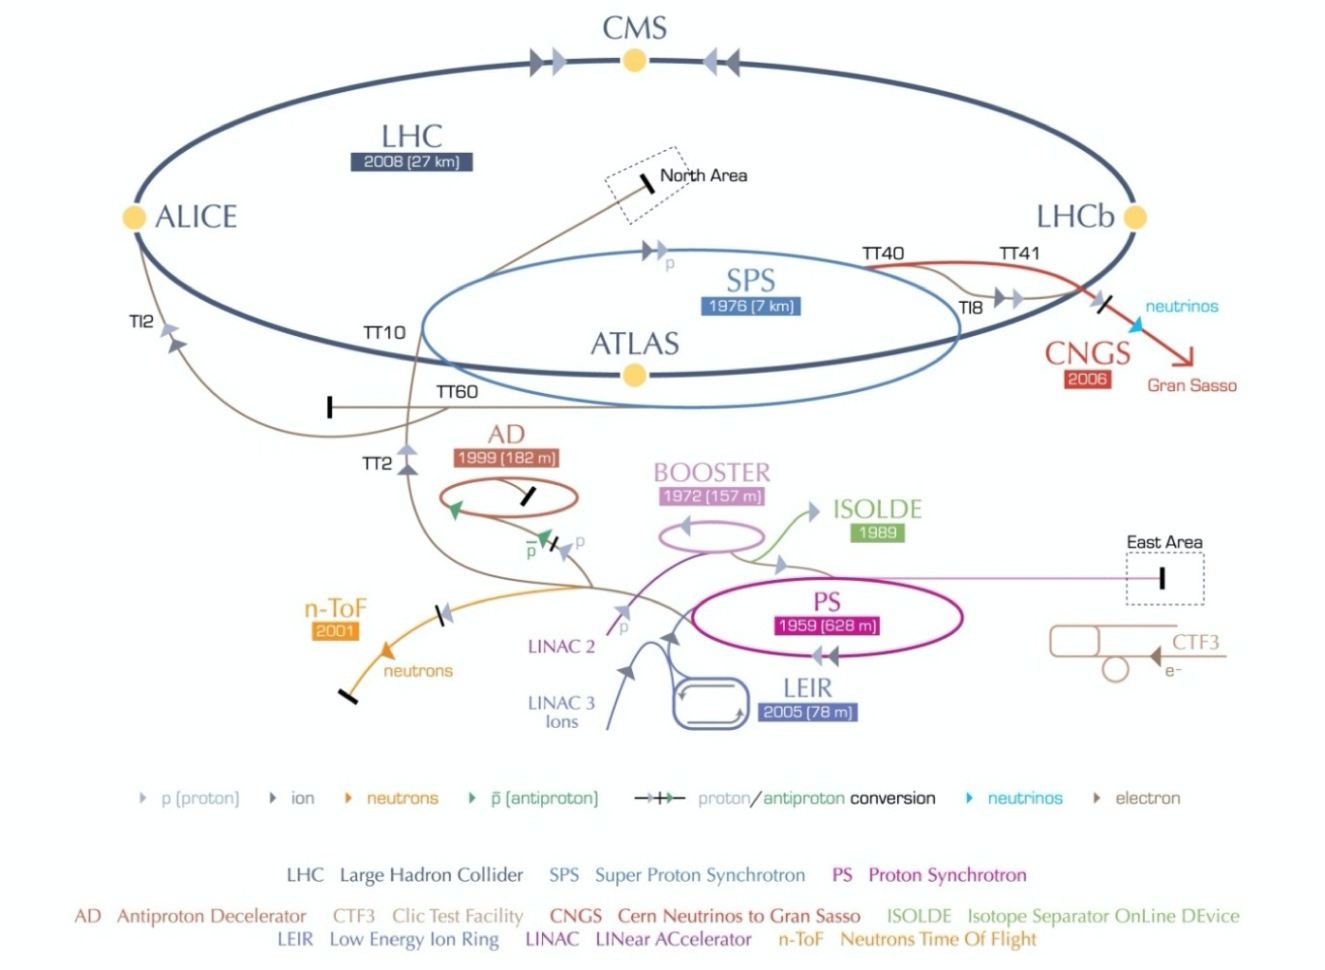
\includegraphics[width=10cm]{LHC_overview}
\caption[LHCの全体像]{LHCの全体像\cite{1-1}}
\label{LHC_overview}
\end{figure}

\section{ATLAS実験}

\subsection{ATLAS検出器}

\begin{figure}[bpt]\centering
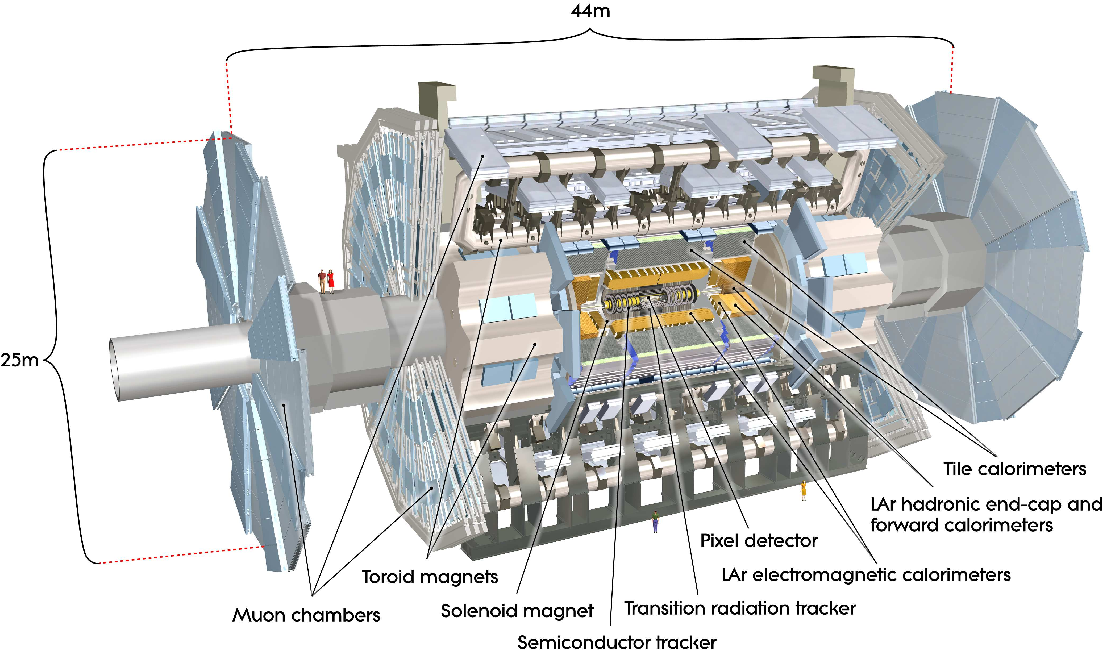
\includegraphics[width=10cm]{atlas_detector}
\caption[ATLAS検出器]{ATLAS検出器\cite{1-2}}
\label{atlas_detector}
\end{figure}

\begin{figure}[bpt]\centering
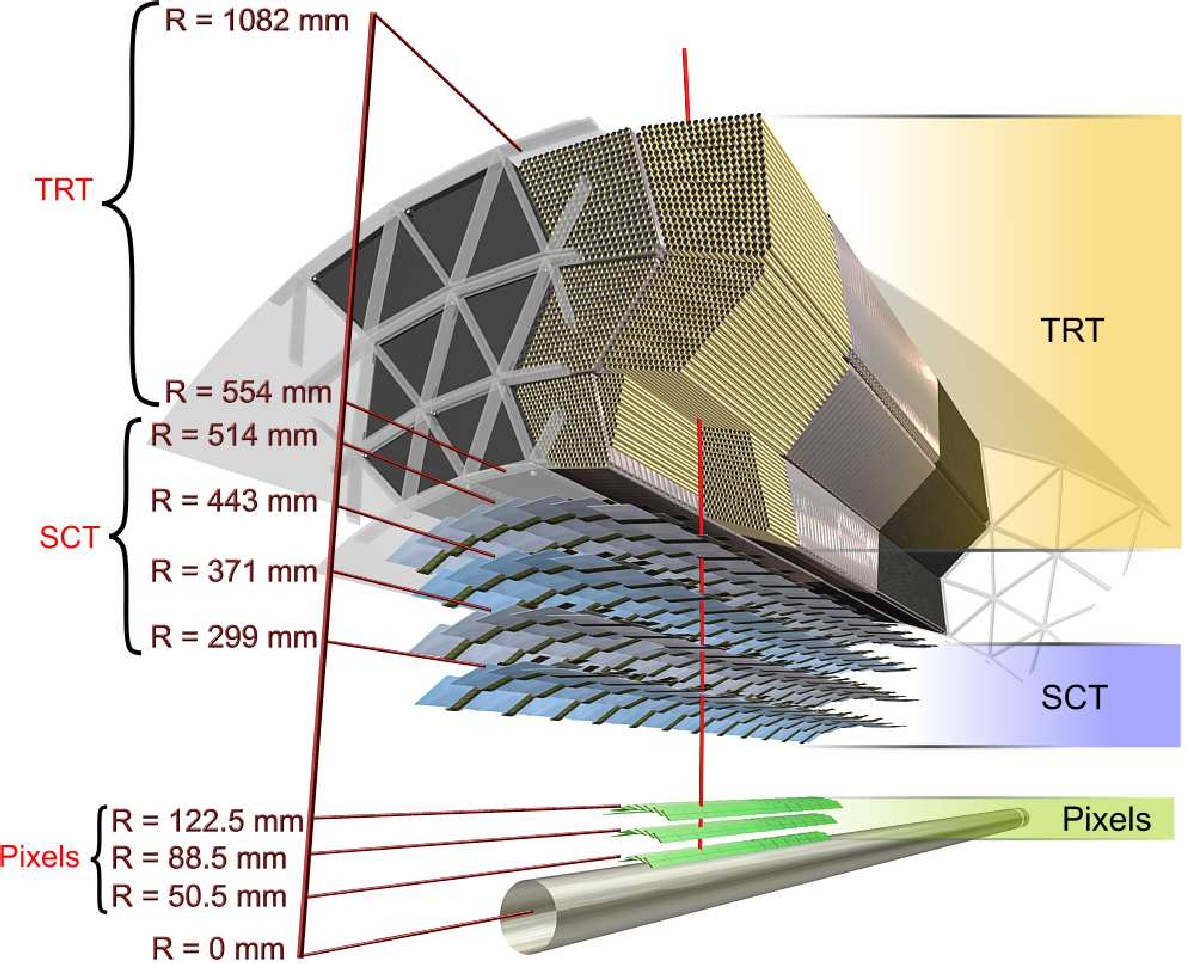
\includegraphics[width=10cm]{atlas_detector_cross_section}
\caption[ATLAS検出器]{ATLAS検出器\cite{1-2}}
\label{atlas_detector_cross_section}
\end{figure}

\subsection{内部飛跡検出器}

\begin{figure}[bpt]\centering
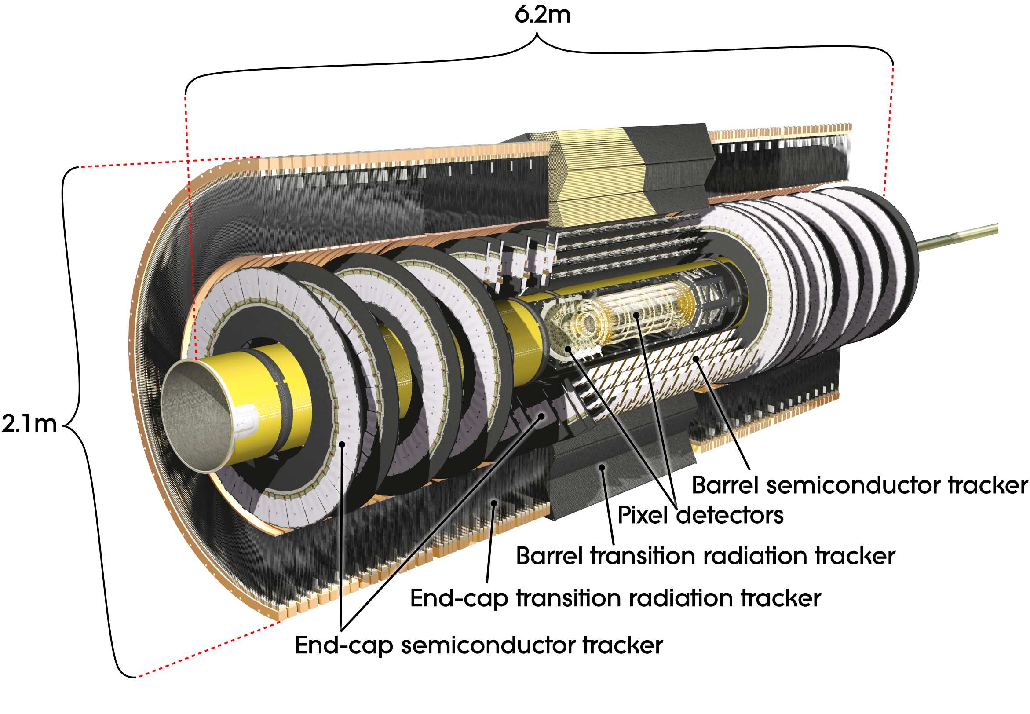
\includegraphics[width=10cm]{inner_detector}
\caption[内部飛跡検出器]{内部飛跡検出器\cite{1-2}}
\label{inner_detector}
\end{figure}

\begin{figure}[bpt]\centering
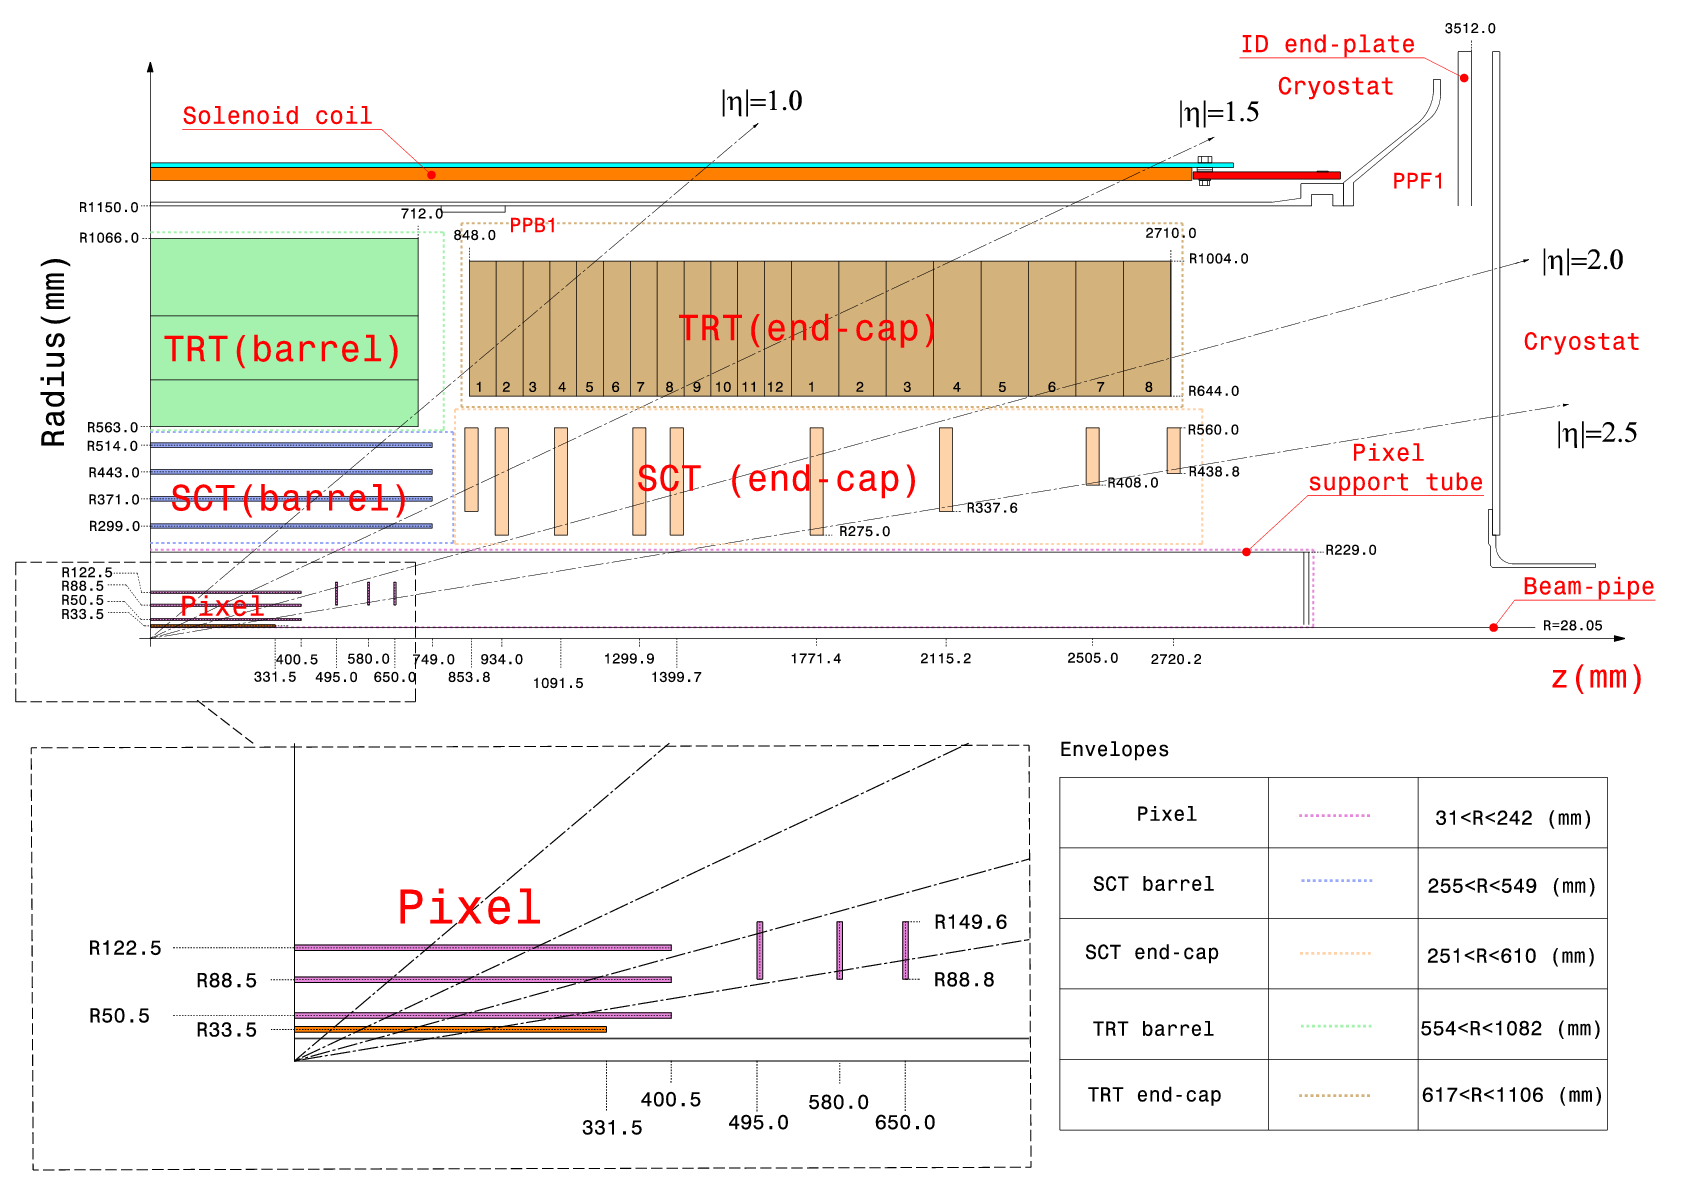
\includegraphics[width=10cm]{inner_cross_section}
\caption[内部飛跡検出器]{内部飛跡検出器\cite{1-2}}
\label{inner_cross_section}
\end{figure}

\subsubsection{ピクセル検出器}

\begin{figure}[bpt]\centering
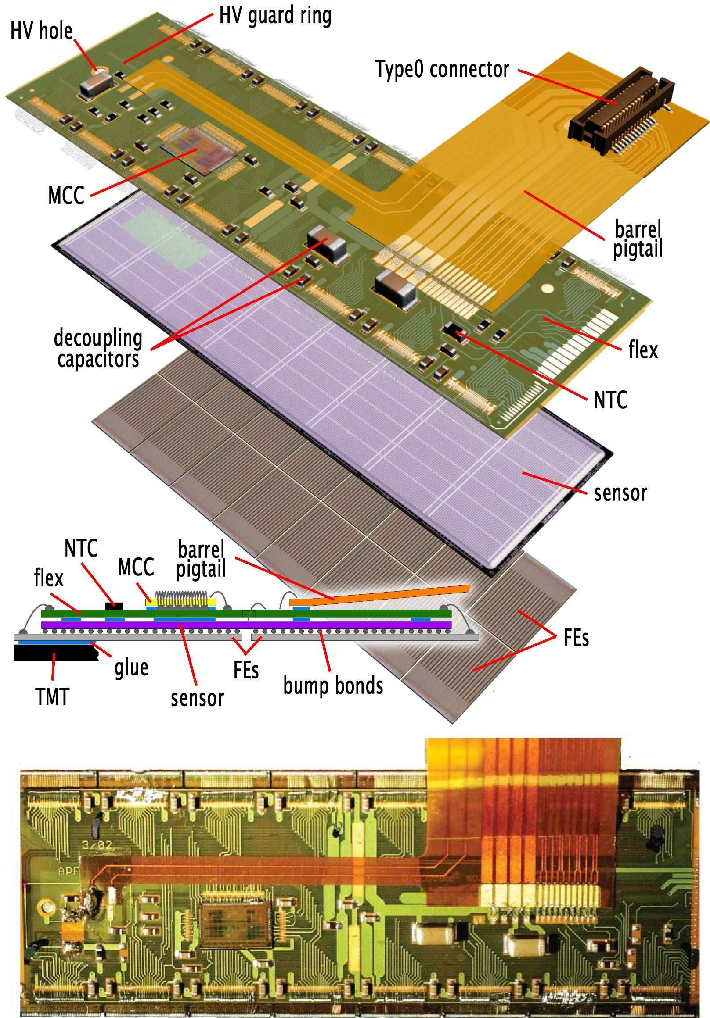
\includegraphics[width=10cm]{pixel_detector}
\caption[ピクセル検出器]{ピクセル検出器\cite{1-2}}
\label{inner_detector}
\end{figure}

\subsubsection{ストリップ検出器}

\begin{figure}[bpt]\centering
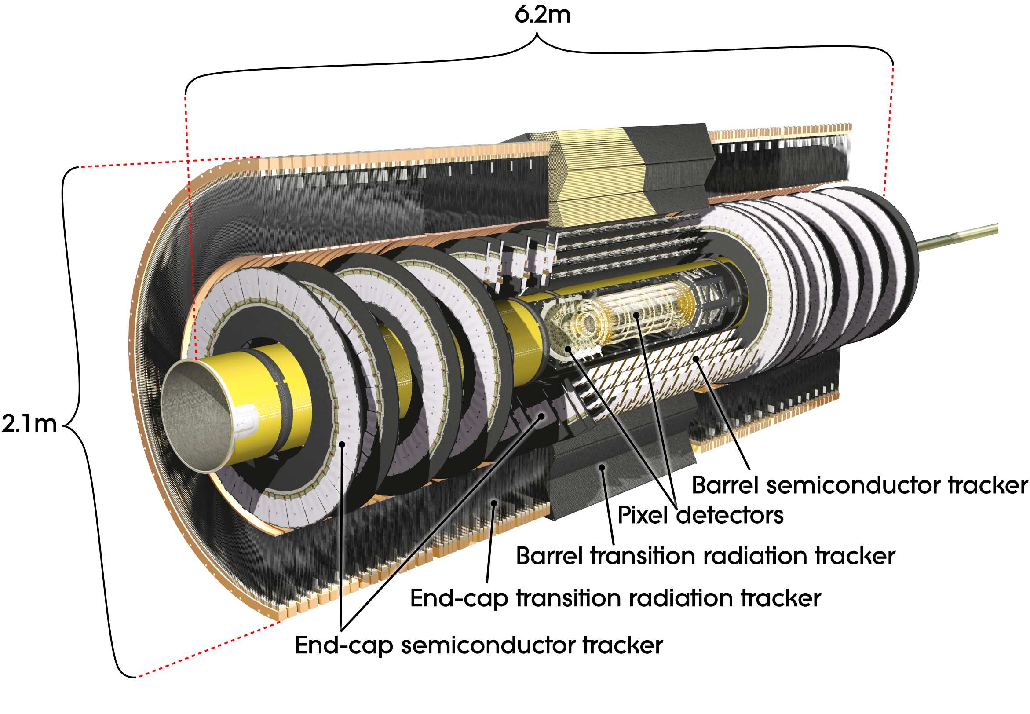
\includegraphics[width=10cm]{inner_detector}
\caption[ストリップ検出器]{ストリップ検出器\cite{1-2}}
\label{inner_detector}
\end{figure}


\section{HL-LHC実験アップグレード計画}
\subsection{概要}
\subsection{内部飛跡検出器のアップグレード}

\begin{figure}[bpt]\centering
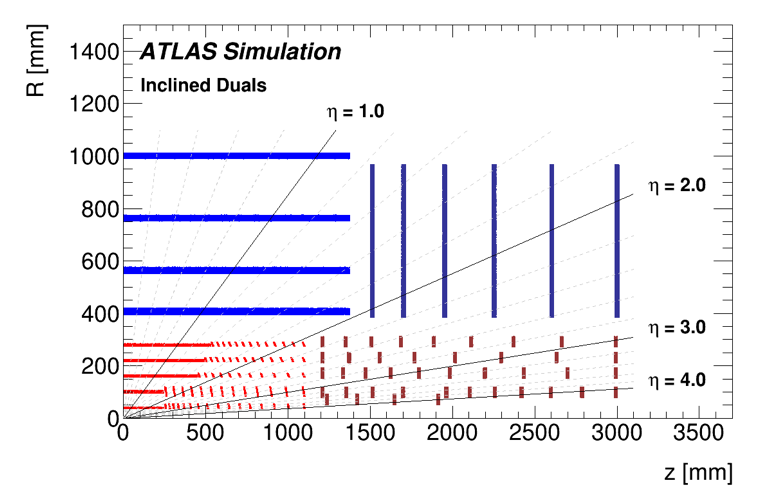
\includegraphics[width=10cm]{itk_cross_section}
\caption[ITkの断面図]{ITkの断面図\cite{1-3}}
\label{itk_cross_section}
\end{figure}

\begin{figure}[bpt]\centering
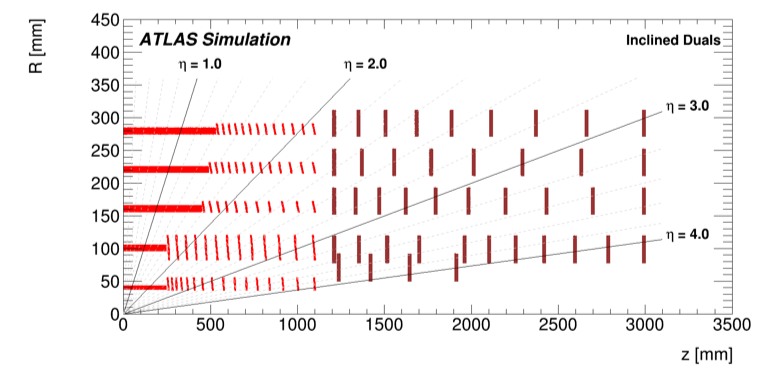
\includegraphics[width=10cm]{itk_pixel_cross_section}
\caption[ITkピクセルの断面図]{ITkピクセルの断面図\cite{1-3}}
\label{itk_pixel_cross_section}
\end{figure}

\subsection{期待される物理}
